%%%%%%%%%%%%%%%%%%%%%%%%%%%%%%%%%%%%%%%%%%%%%%%%%%%%%
%% 导言区
%%%%%%%%%%%%%%%%%%%%%%%%%%%%%%%%%%%%%%%%%%%%%%%%%%%%%

\documentclass[a4paper, zihao=5, UTF8, AutoFakeBold]{ctexart}

%% ===== 排版宏包 =====
\usepackage{pdfpages}
\usepackage{fontspec}
\usepackage{setspace}
\usepackage{titlesec}
\usepackage{fancyhdr}
\usepackage[most]{tcolorbox}
\usepackage{geometry}
\usepackage{tikz}
\usepackage{pgfplots}
\usepackage{amsmath}
\usepackage{amssymb}
\usepackage{graphicx}
\usepackage{caption}
\usepackage{float}
\usepackage{dblfloatfix}
\usepackage{xcolor}
\usepackage{hyperref}
\usepackage{tabularray}
\UseTblrLibrary{booktabs, siunitx}  
\usepackage{etoolbox}
\usepackage{xparse}
\usepackage{chngcntr}
\usepackage{balance}

%%%%%%%%%%%%%%%%%%%%%%%%%%%%%%%%%%%%%%%%%%%%%%%%%%%%%
%% 格式区
%%%%%%%%%%%%%%%%%%%%%%%%%%%%%%%%%%%%%%%%%%%%%%%%%%%%%

%% ===== 参考文献格式设置 =====
\usepackage
[
    backend=biber, 
    style=gb7714-2015, 
    gbnamefmt=uppercase, 
    maxbibnames=3, minbibnames=3, 
    doi=false, 
    eprint=false, 
    url=false,
]{biblatex}
\addbibresource{references.bib}
\AtBeginBibliography{\vspace{-22pt}\zihao{-5}\noindent}
\defbibheading{bibliography}[\refname]{\section*{#1}}


%% ===== 页面设置 =====
\geometry{top=2.5cm, bottom=1.7cm, left=2cm, right=2cm}
\pagestyle{fancy}
\fancyhf{}

%% ===== 字体设置 =====
\setmainfont{Times New Roman}
\setCJKmainfont{SimSun}

%% ===== 行距 段距 栏距 =====
\setstretch{1.08333}
\setlength{\parskip}{0pt}
\setlength{\columnsep}{2em}

%% ===== 标题格式 =====
\titleformat{\section}[block]{\heiti\zihao{-4}}{\thesection}{0.5em}{}
\titleformat{\subsection}[block]{\heiti}{\thesubsection}{0.5em}{}
\titleformat{\subsubsection}[block]{\kaishu}{\thesubsubsection}{0.5em}{}

%% 表格与图像用的半角空格
\DeclareCaptionLabelSeparator{halfspace}{\hspace{0.5em}}

%% ===== 表格格式 =====
\captionsetup[table]{justification=centering, singlelinecheck=false}
\counterwithin{table}{section}
\DeclareCaptionFont{tableCaption}{\zihao{-5}\heiti}
\captionsetup[table]
{
    font       = tableCaption,
    labelsep   = halfspace,
    position   = top,
    justification = centering,
}
\captionsetup[table]{skip = 2.5pt}
\AtBeginEnvironment{tblr}{\zihao{-5}}

%% ===== 图片格式 =====
\captionsetup[figure]{justification=centering, singlelinecheck=false}
\counterwithin{figure}{section}
\DeclareCaptionFont{figureCaption}{\zihao{-5}}
\captionsetup[figure]
{
    font = figureCaption,
    labelsep = halfspace,
    position = bottom,
    justification =  centering,
}

%% ===== 绘图格式 =====
\pgfplotsset
{
    ExperimentStyle/.style=
    {
        axis line style={semithick},
        tick style={semithick},
        scaled ticks=false,
        grid=none,
        legend style=
        {
            font=\zihao{-5},
            draw=none,
            fill=none,
        },
        label style={font=\zihao{-5}},
        tick label style={font=\zihao{-5}},
        every axis plot/.append style=
        {
            black,
            semithick,
            mark=*,
            mark size = 1pt,
        }
    }
}

%%%%%%%%%%%%%%%%%%%%%%%%%%%%%%%%%%%%%%%%%%%%%%%%%%%%%
%% 命令区
%%%%%%%%%%%%%%%%%%%%%%%%%%%%%%%%%%%%%%%%%%%%%%%%%%%%%

\newcommand{\titleZHfont}{\heiti\zihao{-2}}                         %% 中文标题的字体
\newcommand{\authorZHfont}{\kaishu\zihao{4}}                        %% 中文作者字体
\newcommand{\addressZHfont}{\kaishu\fontsize{9pt}{10pt}\selectfont} %% 中文作者单位字体
\newcommand{\abstractZHfont}{\fontsize{9pt}{15pt}\selectfont}       %% 中文摘要字体
\newcommand{\titleENfont}{\bfseries\zihao{3}}                       %% 英文标题的字体
\newcommand{\authorENfont}{\zihao{-4}}                              %% 英文作者字体
\newcommand{\addressENfont}{\zihao{5}}                              %% 英文作者单位字体
\newcommand{\abstractENfont}{\fontsize{10.5pt}{15pt}}               %% 英文摘要字体

%% ===== 封装图片插入命令 =====
\newcommand{\pic}[2]
{
    \begin{figure}[!htbp]
        \centering
        \includegraphics[width=\linewidth]{#1}
        \caption{#2}
    \end{figure}
}

%% ===== 封装绘图中的引线标注命令 =====
%% 用法：\LineLabel{X}{Y}{x}{y}{position}{text}
%% X和Y是被标注的坐标，x和y是标注文本的坐标，position是标注文本的相对位置，text是标注内容
\NewDocumentCommand{\LineLabel}{m m m m m m}
{
    \draw
    (axis cs:#1,#2)
    --
    (axis cs:#3,#4)
    node
    [
        {#5},
        font=\zihao{-5}
    ]
    {#6};
}

%%%%%%%%%%%%%%%%%%%%%%%%%%%%%%%%%%%%%%%%%%%%%%%%%%%%%
%% 导言区结束
%%%%%%%%%%%%%%%%%%%%%%%%%%%%%%%%%%%%%%%%%%%%%%%%%%%%%

%% 以下为论文内容
\begin{document}

%% 封面
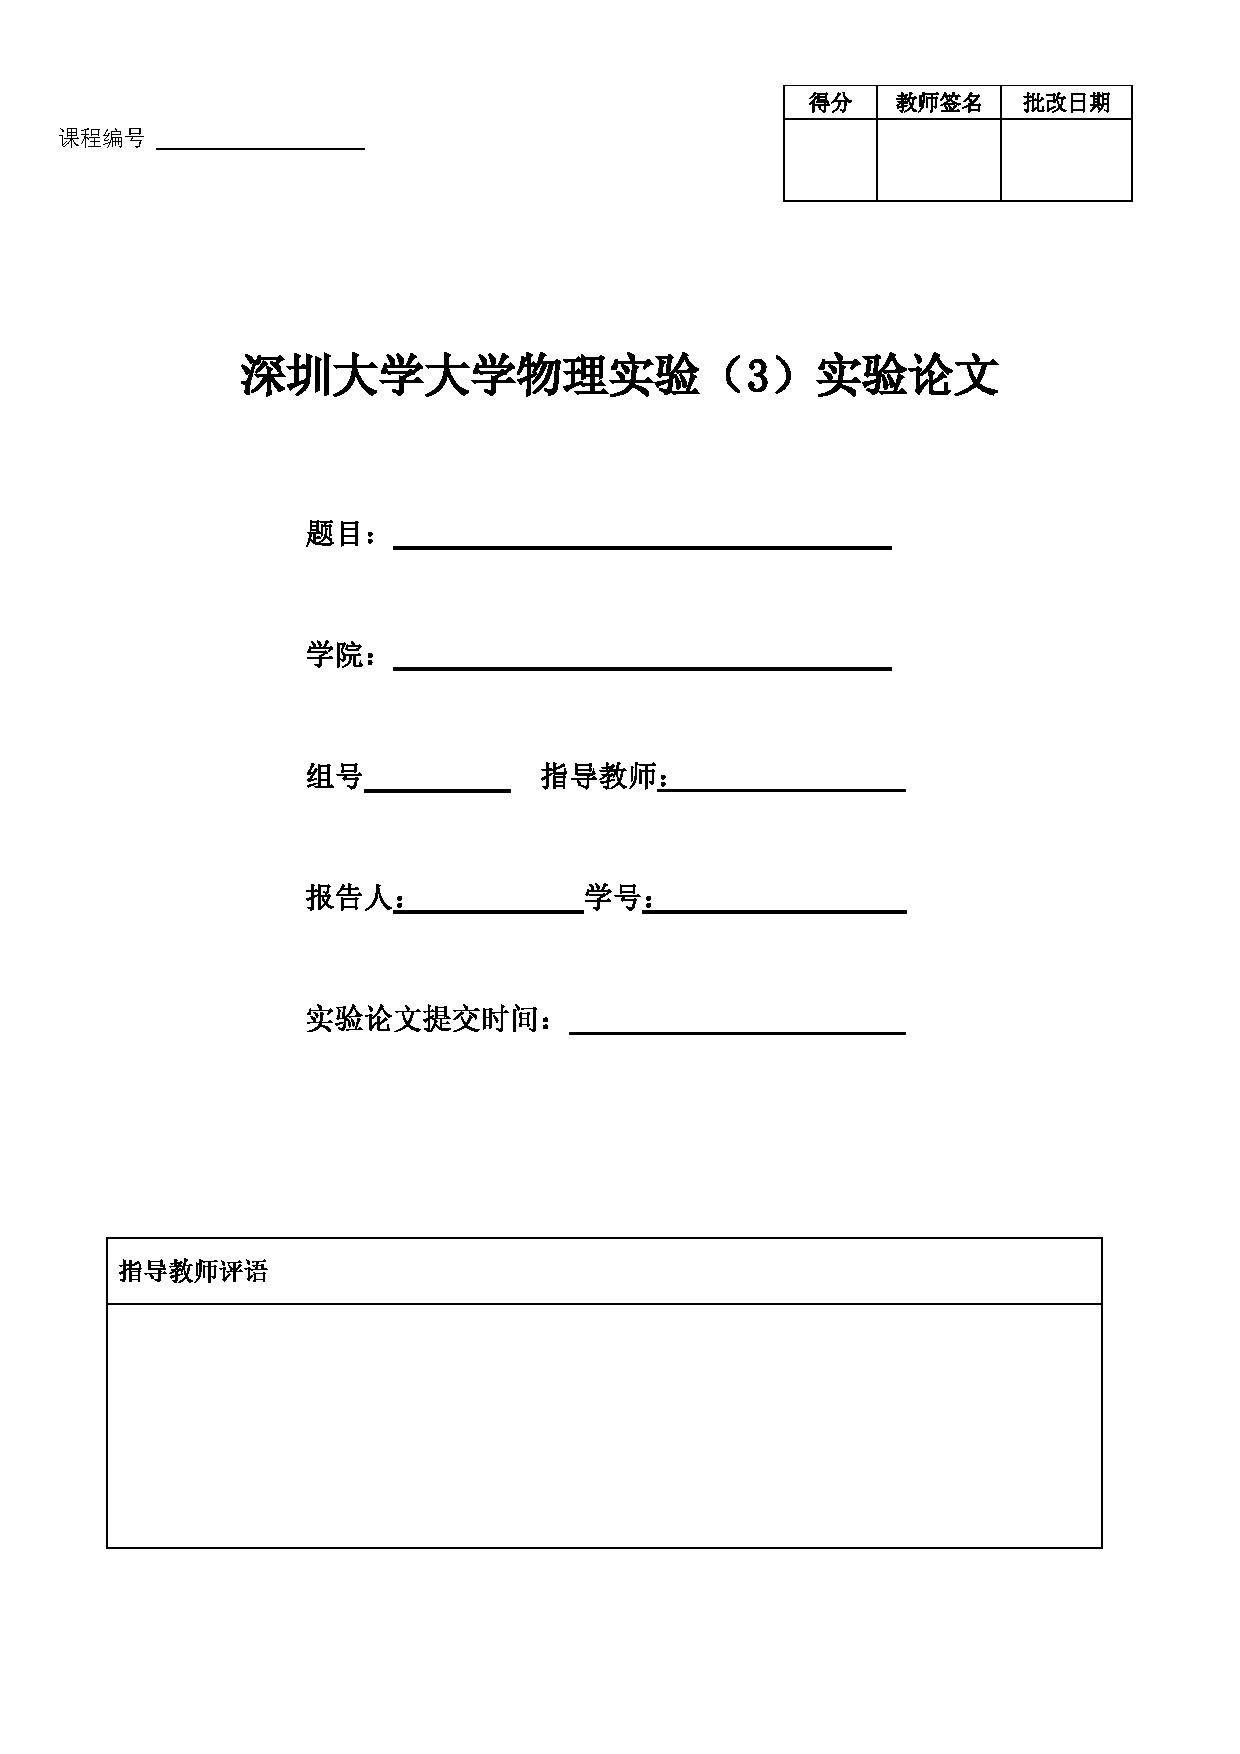
\includepdf{cover/cover.pdf}

\twocolumn
[
%% 中文标题与摘要
\begin{center}
    \vspace{-15pt}
    {\titleZHfont 这里写文章标题} \\
    \vspace{18pt}
    {\authorZHfont 这里写作者姓名} \\
    {\addressZHfont 这里写作者单位} \\
    \vspace{6pt}
\end{center}

\begin{flushleft}
    {\fontsize{9pt}{15pt}\selectfont\heiti 摘{\quad}要：}
    {\abstractZHfont 
                    摘要内容。概括地陈述论文研究的目的、方法、结果、结论，要求200～300 字。应排除本学科领域已成为常识的
                    内容；不要把应在引言中出现的内容写入摘要，不引用参考文献；不要对论文内容作诠释和评论。不得简单重复题名中已有
                    的信息。用第三人称，不使用“本文”、“作者”等作为主语。使用规范化的名词术语，新术语或尚无合适的汉文术语的，可
                    用原文或译出后加括号注明。除了无法变通之外，一般不用数学公式和化学结构式，不出现插图、表格。缩略语、略称、代
                    号，除了相邻专业的读者也能清楚理解的以外，在首次出现时必须加括号说明。结构严谨，表达简明，语义确切。} \\
    {\fontsize{9pt}{15pt}\selectfont\heiti 关键词：}
    {\abstractZHfont 这里写关键词内容} \\
    {\fontsize{9pt}{15pt}\selectfont\heiti 中图分类号：}
    {\abstractZHfont （作者本人填写）}\hspace{3em}
    {\fontsize{9pt}{15pt}\selectfont\heiti 文献标识码：A} \\
\end{flushleft}

%% 英文标题与摘要
\begin{center}
    {\titleENfont Title of the Article} \\
    \vspace{6pt}
    {\authorENfont Author Name} \\
    {\addressENfont Author Affiliation} \\
\end{center}

\begin{flushleft}
    {\abstractENfont{\bfseries Abstract:}
    fulfill here with abstract.\\
    {\bfseries Key Words:}
    fulfill here with Key Words.}\\
\end{flushleft}
]

%% 正文部分
\setlength{\parindent}{2em}

引言内容。引言作为论文的开场白，应以简短的篇幅介绍论文的写作背景和目的，以及相关领域内前人所做的工作和研究概况。
说明本研究与前人工作的关系，目前研究的热点、存在的问题及作者工作的意义。
1、开门见山，不绕圈子。避免大篇幅地讲述历史渊源和立题研究过程。
2、言简意赅，突出重点。不应过多叙述同行熟知的及教科书中的常识性内容，确有必要提及他人的研究成果和基本原理时，只需以引用参考文献的形势标出即可。在引言中提示本文的工作和观点时，意思应明确，语言应简练。
3、引言的内容不要与摘要雷同，也不是摘要的注释。
4、引言要简短，最好不要分段论述，不要插图、列表和数学公式。 

\section{量的书写规则}
正文内容。正文、图表中的变量都要用斜体字母，对于矢量和张量使用黑斜体，只有pH采用正体；使用新标准规定的符号；量的符号为单个拉丁字母或希腊字母；
不能把量符号作为纯数使用；不能把化学符号作为量符号使用，代表物质的符号表示成右下标，具体物质的符号及其状态等置于与主符号齐线的圆括号中[1]。\par
注意区分量的下标字母的正斜体：凡量符号和代表变动性数字及坐标轴的字母作下标，采用斜体字母。\par
正文中引用参考文献的标注方法，在引用处对引用的文献，按它们在论著中出现的先后用阿拉伯数字连续排序，将序号置于方括号内，并视具体情况把序号作为上角标或作为语句的组成部分。\par

\subsection{单位的书写规则}
正文内容。单位符号无例外的采用正体字母[2]。注意区分单位符号的大小写：一般单位符号为小写体，来源于人名的单位符号首字母大写。体积单位升的符号为大写L。\par

\subsubsection{表格的规范化}
正文内容。表格的设计应该科学、明确、简洁，具有自明性。表格应采用三线表，项目栏不宜过繁，小表宽度小于7.5 cm，大表宽度为12～15cm 。
表必须有表序、表题。表中顶线与栏目线之间的部分叫项目栏，底线与栏目线之间的部分叫表身[3]。表身中数字一般不带单位，百分数也不带百分号，应把单位符号和百分号等归并在栏目中。
如果表中栏目中单位均相同，则可把共同的单位提出来标示在表格顶线上方的右端（不加“单位”二字）。表身中同一栏各行的数值应以个位（或小数点），且有效位数相同。
上下左右相邻栏内的文字或数字相同时，应重复写出。

\section{图的规范化}
正文内容。插图可用彩色图。小图宽度小于7.8cm，大图宽度为12～15cm 。图必须有图序、图题。函数图只在靠近坐标线处残留一小段标值短线，其余部分省略。
加注坐标所代表的量及单位（如t/s）。标值排印在坐标外侧，紧靠标值短线的地方；标值的有效数字为3位。图中量的意义要在正文中加以解释。
若有图注，靠近放在图下部，图序、图题的上方。

\section{数学符号和数学式的编排规范}
正文内容。变量、变动附标及函数用斜体字母表示。点、线段及弧用斜体字母表示。在特定场合中视为常数的参数也用斜体字母表示。
对具有特殊定义的函数和值不变的数学常数用正体字母表示[4]。具有特殊定义的算子也用正体字母表示。矩阵符号用大写的黑斜体字母表示，矩阵元素用白斜体字母表示。\par
公式及公式中的符号说明尽量接排以节省版面。把带有复杂上角标的指数函数 写成 。公式的主体应排在同一水平线上；繁分式的主辅线要分清。长公式在运算符号后回行；
长分式转行时，先将分母写成负幂指数的形式，然后转行；矩阵和行列式不能转行。矩阵元素包含式子时，每一列应以中心线上下对齐，行要左右排齐；
元素为单个字母或数字时，每列应使正负号对齐。对角矩阵中对角元素所在的列应明显区分，不能上下重叠[5]。\par
简单的和常识性的运算公式和推导过程不要列写。\par

\section{结论}
正文内容。结论不应是正文中各段小结的简单重复，它应以正文中的实验或考察得到的现象、数据的阐述分析为依据，完整、准确、简洁地指出以下内容：
1）由对研究对象进行考察或实验得到的结果所揭示的原理及其普遍性；
2）研究中有无发现例外或本论文尚难以解释和解决的问题；
3）与先前发表过的研究工作的异同；
4）本文在理论上和实用上的意义及价值；
5）进一步深入研究本课题的建议。

实验结果\cite{paper1}。

教材参考\cite{book1}。

相关研究见\cite{thesis1}。

%% 参考文献区
\balance  %%请把该命令放在最后一页内容的起始位置
\vspace{-6pt}
\printbibliography
[
    heading=bibliography,
    title={参考文献}
]

\end{document}



